\chapter{ Констукторский раздел}
\label{cha:design}
    В данном разделе будет рассмотрена схема алгоритма, требования к функциональности ПО,
    и опредены способы тестирования.
    
    \section{Разработка алгоритма}
        Ниже будет представлена схема алгоритма обратной трассировки лучей.

        Алгоритм обратной трассировки лучей (рисунок \ref{schema:rtx});


    \begin{figure}[h!]
        \centering
            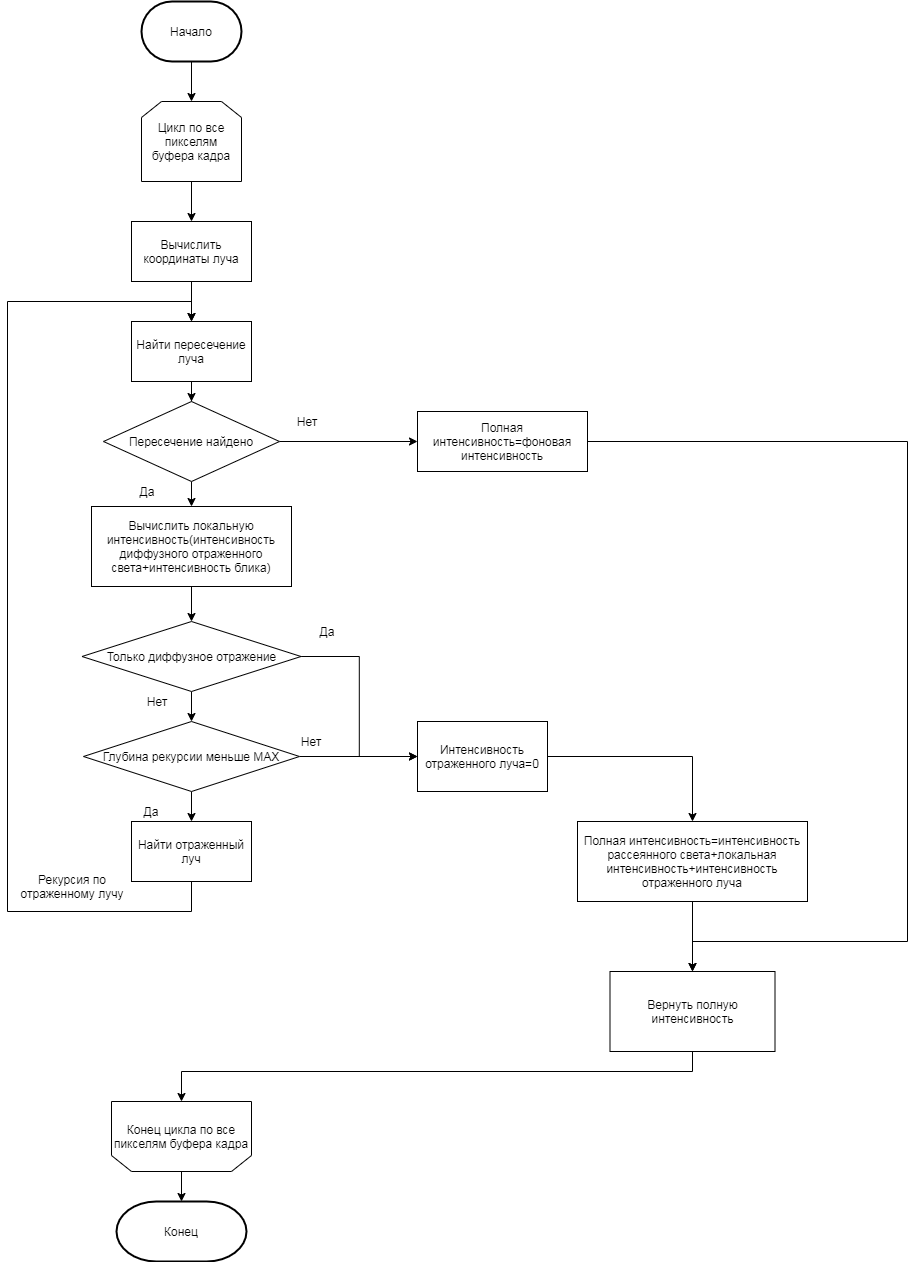
\includegraphics[scale=1.0]{rtx.png}
            \caption{Схема алгоритма обратной трассировки лучей}
            \label{schema:rtx}
    \end{figure}

    \section{Параллельные вычисления}
Распрараллеливание программы должно ускорять время работы. Это достигается за счет реализации в узких участках (напимер в циклах с большим количеством независимых вычилений).

В предложенном алгоритме данным участком будет являться основной двойной цикл вычислений.
Данный блок программы как раз предлагается распараллелить.


    \section{Требования к функциональности ПО}
        В данной работе требуется обеспечить следующую минимальную функциональность оконного приложения:
        \begin{enumerate}
	\item обеспечить ввод координат положения камеры наблюдателя;
	\item обеспечить ввод значения угла, на который необходимо повернуть камеру наблюдателя относительно оси oY;
            \item обеспечить вывод полученного с помощью алгоритма обратной трассировки лучей изображения;
            \item обеспечить вывод замеров времени работы алгоритма обратной трассировки лучей.
        \end{enumerate}

    \section{Методы тестирования}
    Тестирование ПО будет проводиться методом черного ящика.

\newpage